\bdichapter{Paolo Chiocchetti}{Der Niedergang der radikalen Linken in Italien}{}{}

\begin{multicols*}{2}

\noindent Lange galt Italien als Hochburg der radikalen Linken Westeuropas sowie als politisches und intellektuelles Vorbild für linke Kräfte anderer Länder. Vor 1989 war die Italienische Kommunistische Partei (Partito Comunista Italiano, PCI) die stärkste kommunistische Partei diesseits des Eisernen Vorhangs und stärker als die Summe sämtlicher Schwesterparteien (Vittoria 2006). Auf ihrem Höhepunkt im Jahre 1976 konnte sie 12,6 Millionen Wähler (34,4 Prozent), 1,8 Millionen Mitglieder, ein mächtiges Netzwerk von Vorfeldorganisationen und Regierungsstellen in mehreren Regionen und Großstädten vorweisen. Die Gruppen der ‚neuen Linken‘, unter anderem die Partei Proletarische Demokratie (Democrazia Proletaria, DP), waren zwar kleiner aber seit 1976 kontinuierlich im Parlament vertreten und bei der Jugend, in intellektuellen Kreisen und in außerparlamentarischen Mobilisierungen durchaus einflussreich (Balestrini und Moroni 1997; Pucciarelli 2011). 

Historische Perioden wie der antifaschistische Widerstand (1943–1945) oder das ‚lange Achtundsechzig‘ (1968–1977) sahen die Entstehung von starken und radikalen linksgeführten Massenbewegungen, die zwar die Macht nicht ergreifen konnten, aber oft wichtige soziale und politische Erfolge erzielten. Auf intellektueller Ebene dienten die Werke von Antonio Gramsci und seinen italienischen Nachfolgern, von Operaismus-Theoretikern wie Antonio Negri und von weiteren neomarxistischen und kritischen Denkern weltweit als Inspiration. Auch nach dem Fall des Ostblocks wurde die Entwicklung der Partei der Kommunistischen Wiedergründung (Partito della Rifondazione Comunista, PRC) oft als Erfolgsgeschichte gewertet (Bertolino 2004). Obwohl sie 1996 nur 3,2 Millionen Stimmen (8,6 \%) und 130.000 Mitglieder für sich gewinnen konnte, schien die Partei für viele externe Beobachter die Machbarkeit einer Erneuerung des europäischen Kommunismus zu beweisen. Sie wurde später als Mitgründer des Genua Sozialforums (2001), des Europäischen Sozialforums (2002) und der Partei der Europäischen Linken (2004) zu einer treibenden Kraft der internationalen Vernetzung der globalisierungskritischen Linken.

Von dieser Erfolgsgeschichte bleiben heute nur Trümmer. Bei den Parlamentswahlen in Italien 2008 verfehlten alle linken Listen die Vier-Prozent-Hürde. Die PRC spaltete sich in mehrere konkurrierende Organisationen, die meist in der Bedeutungslosigkeit versanken. Nur eine von ihnen schaffte seit 2013 dank Wahlbündnissen mit größeren Mitte-Links-Verbündeten den Wiedereinzug ins Parlament, verlor aber fortschreitend an Ausstrahlungswirkung und Kohärenz. Ferner konnte keine dieser schwachen, demoralisierten Gruppen einen wirksamen außerparlamentarischen Widerstand gegen die Wirtschaftskrise und die durch aufeinanderfolgende Regierungen betriebene Sozialabbaupolitik zu leisten. Bei der Neuwahl am 25. September 2022 war wenig Veränderung zu erwarten. Das Linksbündnis Unione Popolare (Volksunion) scheiterte mit 1,43 \% der Wählerstimmen, die links-grüne Alleanza Verdi e Sinistra zog mit 3,6 \% ins Parlament ein.

Die Etappen dieses Scheiterns sind leicht zu skizzieren. Schwieriger ist es, ihre tieferen Ursachen zu beleuchten. Letztlich scheinen die Perspektiven für einen möglichen Aufschwung derzeit düster zu sein. Der vorliegende Aufsatz wird versuchen, diese Fragen punktuell zu behandeln und plausible Antworten anhand der italienischen und vergleichenden empirischen Daten zu liefern.

\section{Etappen eines Niedergangs: 1977–2021 }

Der Niedergang der radikalen Linken in Italien kann anhand ihrer Wahlergebnisse beschrieben werden (Abbildung 1, Tabelle 1). Die Angaben beziehen sich auf den Anteil der gültigen Stimmen bei Parlamentswahlen (Camera) von 1977 bis 2021. Neben den italienischen Ergebnissen werden als Vergleichswert die Gesamtergebnisse in zwanzig westeuropäischen Staaten – Belgien, Dänemark, Deutschland, Finnland, Frankreich, Griechenland, Irland, Island, Italien, Luxemburg, Malta, Niederlande, Norwegen, Österreich, Portugal, Schweden, der Schweiz, Spanien, dem Vereinigten Königreich und Zypern – angeführt. Diese umfassen mehr als 300 einzelne Parteien oder Wahllisten, die zwar unterschiedlich in Bezug auf ihre Größe, Herkunft, Ideologie und Radikalität sind, aber nachvollziehbar als Teil derselben Parteienfamilie – der sogenannten ‚radikalen Linken‘ – betrachtet werden können. Obwohl er nicht unstrittig ist,  beschreibt der Begriff ‚radikale Linke‘ oder ‚Linke‘ eine Reihe von Parteien, die sich deutlich von den sozialdemokratischen und grünen Parteienfamilien durch ihre theoretische Opposition zum ökonomischen Liberalismus und Kapitalismus, ihren ideellen Anspruch auf Vertretung der Interessen der Arbeiterklasse, ihr auf sozialen Schutz, Umverteilung und Emanzipation basiertes Programm und ihre internationalen Verbindungen (insbesondere die ‚Fraktion Die Linke im Europäischen Parlament – GUE/NGL‘) unterscheiden (Chiocchetti 2017; Calossi 2016; March und Mudde 2005; De Waele und Seiler 2011). Während das Streben nach alternativen sozialistischen Gesellschaftsmodellen (z.B. Realsozialismus, demokratischem ‚Eurokommunismus‘ oder klassenlosem Kommunismus) vor 1989 ideologisch üblicherweise im Vordergrund stand, hat die zeitgenössische Linke dieses Ziel heruntergespielt und zum Teil aufgegeben und ist vor allem durch die Wiederaufnahme gemäßigter demokratischer, sozialer und ökologischer Reformen gekennzeichnet. Dadurch lassen sich vier deutlich definierten Phasen abbilden (Chiocchetti 2017, 2021; Daiber u. a. 2010; Hildebrandt u. a. 2021; Kioupkiolis und Katsambekis 2019; March 2012).

In der ersten Phase (1977 bis 1988) war die radikale Linke in Westeuropa insgesamt noch ziemlich stark, verlor aber allmählich an Kraft. In Italien blieb ihr Niveau außergewöhnlich hoch, weil sie die Krisen der 1950er Jahre (anders als in Nordeuropa) und der 1980er Jahre (anders als in Südeuropa) viel besser verkraftet hatte. Trotz einer langsamen Erosion seit der im Jahr 1976 erreichten Marke von 36,0 \% gewann sie 1987 noch 28,3 \% der Stimmen.

In der zweiten Phase (1989 bis 1993) brach diese Parteienfamilie in Westeuropa zusammen, als mehrere Parteien sich zur Sozialdemokratie oder zur politischen Ökologie bekannten und die übriggebliebenen durch den Zusammenbruch des real existierenden Sozialismus destabilisiert wurden. In Italien war der Sturz abrupter und brutaler. 1989 entschied die PCI-Führung, den Namen und die Natur der Partei zu ändern, rief 1991 eine formell ‚quasi-sozialdemokratische‘, inhaltlich sozialliberale Kraft ins Leben und rückte rasch nach rechts. 

\begin{table*}
    \caption{Wahlergebnisse linker Parteien in Italien (\% der gültigen Stimmen)}
    \begin{tabular}[h]{l|l|l|l|l|l|l|l|l|l}
        & 1987 & 1992 & 1994 &  1996 & 2001 & 2006 & 2008 & 2013 & 2018\\\hline
        Gesamtsumme & 28.3 & 5.6  & 6.1  & 8.6   & 6.7  & 8.0  & 4.4  & 5.7  & 5.0 \\
        PCI & 26.5 &   &   &    &   &   &   &   &  \\
        DP & 1.7 &   &   &    &   &   &   &   &  \\
        PRC & & 5.6  &  6.1 &  8.6  &  5.0 & 5.7  &  (SA) & (RC)  & (PaP)  \\
        PdCI/PCdI/PCI & 1.7 &   &   &    & 1.7  & 2.3  &  (SA) & (RC)  & (PaP) \\
        SA (Wahlbündnis) & 1.7 &   &   &    &   &   & 3.1  &   &  \\
        RC (Wahlbündnis) & 1.7 &   &   &    &   &   &   & 2.2  &  \\
        PaP (Wahlbündnis) & 1.7 &   &   &    &   &   &   &   & 1.1 \\
        SEL/SI & 1.7 &   &   &    &   &   &   &  3.2 & (LeU) \\
        LeU (Wahlbündnis) & 1.7 &   &   &    &   &   &   &   & 3.5 \\
        Sonstige & 0.0 &   &   &    & 0.0 &   & 1.3 & 0.3 &  0.4\\
    \end{tabular}
\end{table*}

Die sich daraus ergebende Partei – zuerst als PDS und später als DS benannt – verschmolz 2007 mit christdemokratischen und zentristischen Kräften in die Demokratische Partei (Partito Democratico, PD). Sie wurde insgesamt fast 17 Jahre lang Regierungskraft in Mitte-Links-Koalitionen und lagerübergreifenden Koalitionen und war mitverantwortlich für die Zerstörung des Nachkriegssystems von dirigistischer Wirtschaftspolitik, redistributiver Sozialpolitik, arbeitnehmerfreundlichen Arbeitsbeziehungen und Konsensdemokratie (Fifi 2022; Guiso 2020).  Mehrere linke Strömungen schlossen sich 1991 zur neokommunistischen PRC zusammen, erhielten aber nur 5,6 \% der Stimmen bei der Wahl 1992.

In der dritten Phase (1994 bis 2008) schwankte diese Parteienfamilie in Westeuropa zwischen Hoffnung und Enttäuschung auf einem leicht aufsteigenden aber relativ niedrigen Wahlniveau. Die Ergebnisse in Italien fielen ähnlich bzw. leicht höher aus. Am Anfang wuchs die PRC von 5,6 \% (1992) auf 8,6 \% (1996). Die durch das neue Mehrheitswahlsystem und Parteiensystem geförderte Zusammenarbeit mit Mitte-\-Links-\-Kräften wurde aber zum Zankapfel und verursachte immer wieder innere Konflikte, Abspaltungen und Wahlverluste. Die Partei wechselte mehrmals zwischen Wahlbündnissen und Alleingang sowie zwischen Opposition (1995–1996, 1998–2001), externer Tolerierung (1996–1998) und direkter Beteiligung (2006–2008) an Mitte-\-Links-\-Regierungen. 

Gemäßigte Strömungen verließen die Partei im Jahr 1995 (Bewegung der Einheitskommunisten, Movimento dei Comunisti Unitari, MCU) und im Jahr 1998 (Partei der italienischen Kommunisten, Partito die Comunisti Italiani, PdCI); kleinere radikale Gruppierungen machten dergleichen in den Jahren 1996–1998 und 2006–2008. Die \looseness=1 Gesamtergebnisse dieser Parteien fielen auf 6,7 \% (2001) und 8,0 \% (2006). Letztendlich schlossen sich verschiedene linke und Mitte-Links-Kräfte zum Wahlbündnis Die Linke – Der Regenbogen (La Sinistra – L’Arcobaleno, SA) zusammen, das 2008 mit 3,2 \% eine katastrophale Niederlage erlitt und den Einzug ins Parlament verpasste.

\begin{figure*}
    \caption{Wahlergebnisse linker Parteien in Westeuropa, 20 Länder (\% der gültigen Stimmen)}
    \centering
    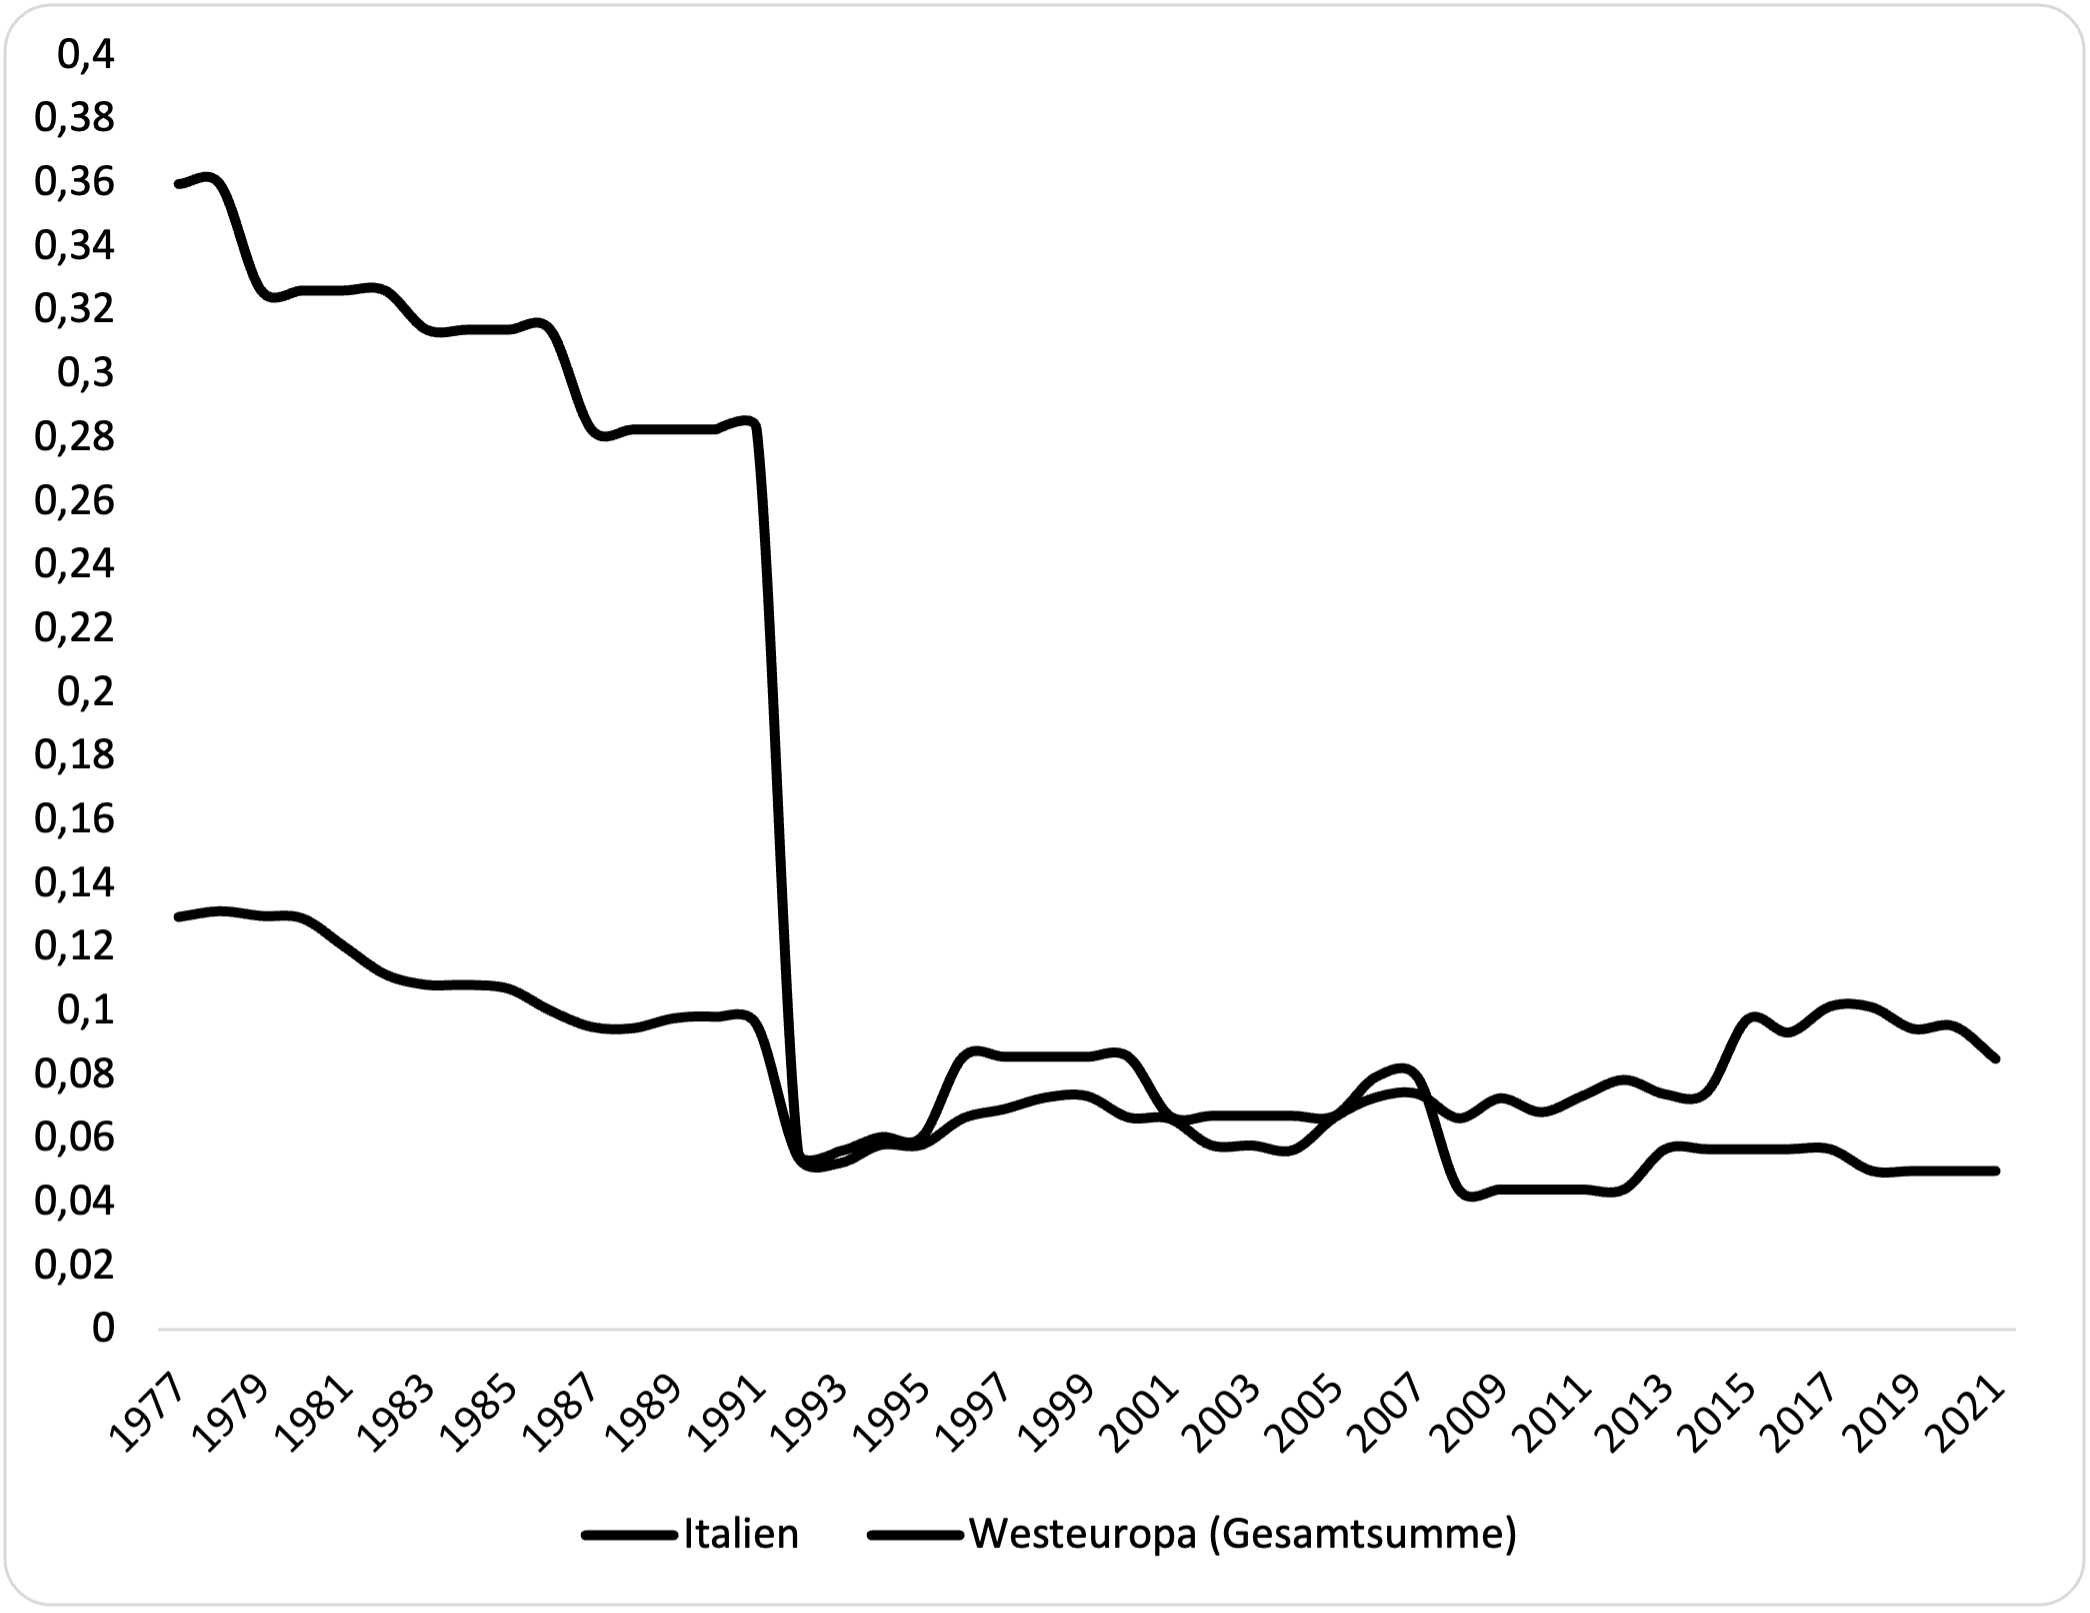
\includegraphics[scale=0.7]{../Bilder/grafik-wahlergebnisse.png}
\end{figure*}

In der vierten Phase (2009–2021) erlebte die europäische Linke in Westeuropa einen starken, wenn auch geographisch ungleichmäßigen, Aufschwung. Ihre Gesamtergebnisse stiegen über das Niveau von 1989 bis zu einem Höhepunkt von 10,2 \% im Jahr 2017. Nach der Weltfinanzkrise feierten alte und neue Parteien eklatante Wahlerfolge in Griechenland (45,0 \%), Spanien (22,6 \%), Portugal (20,7 \%), Irland (27,6 \%) und Frankreich (14,6 \% bei den Parlamentswahlen, aber 21,3 \% bei den Präsidentschaftswahlen). Gleichzeitig erlebten auch einige sozialdemokratische Parteien eine linke Erneuerung: insbesondere die britische Labour Party, die 2017 mit Jeremy Corbyn 40,0 \% der Stimmen erhielt und eine knappe Niederlage erlitt. Im starken Gegensatz dazu blieb die italienische Linke sehr schwach. Die Gesamtergebnisse stiegen zwar leicht von 4,4 \% (2008) auf 5,7 \% (2013) und 5,0 \% (2018), waren aber auf mehrere konkurrierenden Gruppierungen verteilt und zum guten Teil dem Beitrag von Wahlbündnissen mit nichtradikalen sozialdemokratischen, grünen und sonstigen Kräften zu verdanken. Insgesamt ist die Wählerschaft von Organisationen, die sich ausdrücklich als Erben der Geschichte der PCI und PRC, sowie als Teil der zeitgenössischen radikalen Linken verstehen, auf höchstens 2–3 \% geschrumpft. Die Entwicklung der einzelnen Kräfte lässt sich nicht leicht zusammenfassen, da sie wiederholt ihren Namen änderten, Abspaltungen und Fusionen erlebten und zumeist nicht eigenständig zur Wahl antraten. Eine größere rechte Strömung um Nichi Vendola und Nicola Fratoianni verließ 2009 die PRC und gründete mit weiteren Partnern eine neue Partei, zuerst als Linke Ökologie Freiheit (Sinistra Ecologia Libertà, SEL) und heute als Italienische Linke (Sinistra Italiana, SI) bekannt. Diese Partei schaffte 2013 als PD-Verbündeter den Wiedereinzug ins Parlament mit 37 Abgeordneten, verlor aber diese Abgeordneten schrittweise durch scharenweise Austritte und schlechte Wahlergebnisse wieder: 2017 blieben nur siebzehn Abgeordnete, 2018 drei Abgeordnete, und 2021 ein Abgeordneter übrig. Bei der folgenden Wahl trat sie als Teil eines rot-grünen Wahlbündnisses an. Die 2018 treibende Kraft innerhalb des LeU-Wahlbündnisses, die PD-Abspaltung Artikel Eins (Articolo Uno, Art.1), identifizierte sich immer als Teil der sozialdemokratischen Parteienfamilie und trat 2022 wieder innerhalb der PD-Wahlliste an. Die fortbestehende PRC um Paolo Ferrero und Maurizio Acerbo versuchte eine Zusammenarbeit der oppositionellen Linken zu ermöglichen; die meist kurz vor Wahlen unter unterschiedlichen Bezeichnungen ins Leben gerufenen Wahlbündnisse blieben jedoch stets erfolglos. Die letzte Verkörperung dieser Strategie, die Volksunion (Unione Popolare, UP), wurde schon in Umfragen auf 1 \% geschätzt. Der Wahlerfolg blieb auch 2022 für sonstige radikalere Kräfte aus. Verschiedene trotzkistische Gruppen gewannen 1 \% bei der Wahl im Jahr 2008, aber nur 0,1 \% bei der Wahl im Jahr 2018 und traten diesmal nur in wenigen Wahlkreisen an. Die orthodoxe Kommunistische Partei um Marco Rizzo (Partito Comunista, PC) wuchs hingegen von 0,3 \% bei der Wahl 2018 auf 0,9 \% bei der Europawahl 2019 und trat diesmal innerhalb des euroskeptischen und impfkritischen Wahlbündnisses Italia Sovrana e Popolare (ISP) an, das im September 2022 auf 1,2 \% kam.

\section{Unmittelbare und tiefere Ursachen}

\noindent Zusammengefasst sind der Rückgang und die heutige Schwäche der italienischen Linken auf zwei Schlüsselmomente zurückzuführen: einerseits auf den Wechsel der PCI zur Sozialdemokratie nach 1989, die ihr die überwiegende Mehrheit der Wähler, Mitglieder und Ressourcen raubte, andererseits auf die katastrophale Wahlniederlage im Jahr 2008, die ihre parlamentarische Vertretung, Medienpräsenz und staatliche Finanzierung vernichtete und eine spätere Erholung schwermachte. Obwohl sich viele unmittelbare und tiefere Faktoren dafür identifizieren lassen, die für diese Entwicklung mit einiger Wahrscheinlichkeit mitverantwortlich sein könnten, ist ihre tatsächliche Kausalität, ihr relatives Gewicht und ihre historische Notwendigkeit oft schwer einzuschätzen.

In den 1980er und frühen 1990er Jahren war die radikale Linke europa- und weltweit auf dem Rückzug. Dies lässt sich allgemein mit drei allgemeinen Faktoren erklären: (1) die Erosion und Umstrukturierung der industriellen Arbeiterklasse durch strukturellen Wandel, gewerkschaftliche Niederlagen und politische Maßnahmen, die die Kernwählerschaft der Linken schwächten; (2) der Verlust an materieller und ideologischer Anziehungskraft der sozialistischen Planwirtschaften, die zunehmend an niedrigen Wachstumsraten und Warenmangel litten, politisch abschreckender wurden (so durch die chinesische Kulturrevolution, die kambodschanischen Roten Khmer, die Hungersnot im Derg-Äthiopien sowie die Zerschlagung von Solidarność in Polen) und letztendlich nach dem Jahr 1989 weitgehend zusammenbrachen; sowie (3) die Abwanderung von Parteieneliten und Aktivisten durch Kooptation, Demoralisierung und Repression. Diese Faktoren waren auch in Italien vorhanden, führten aber eher zu einer subtilen Veränderung der sozialen und ideologischen Zusammensetzung der PCI als zu Wahlverlusten, da sie als außergewöhnlich große, glaubwürdige und nicht eng mit dem Realsozialismus verbundene linke Oppositionskraft noch von radikalen und gemäßigten Wählern unterstützt werden konnte und ihr engster Konkurrent, die sozialistische Partei, zu schwach und regierungsnah war, um eine ernsthafte Alternative zu bieten. Ihr abrupter Wandel 1989–1990 zu einer postkommunistischen, gemäßigten linken Kraft (Liguori 2009) war aus vergleichender Perspektive wenig überraschend, da die meisten osteuropäischen und mehrere westeuropäische Schwesterparteien den gleichen Weg gingen (Botella, Fernández 2003; Bozóki, Ishiyama 2002). Ihre spätere Wandlung in eine sozialliberale Partei (Bellucci u. a. 2000; Giannetti, Mulé 2006; Natale, Fasano 2017), die politische Inhalte und Klasseninteressen vertritt, die kaum mit jenen der traditionellen sozialistischen Arbeiterbewegung zu tun haben, ist allerdings ideologisch unverständlich, spiegelt aber die allgemeine Entwicklung postkommunistischer und sozialdemokratischer Parteien wider (De Waele u. a. 2013; Gethin u. a. 2022; Nachtwey 2009) und lässt sich zum Teil materialistisch durch die veränderten Interessen der Parteieneliten und der gesellschaftlichen Ober- und oberen Mittelschichten erklären. Letztlich war auch zu erwarten, dass alte oder neue linke Kräfte versuchen würden, die daraus entstandene Vertretungslücke zu füllen und die Sehnsucht nach sozialer Gerechtigkeit und nach dem Wohlfahrtsstaat neu zu verkörpern (Chiocchetti 2017), in Italien war es die PRC. Zugleich ist nicht völlig klar, warum letztere nicht einen größeren Teil der gesellschaftlichen und organisatorischen Verankerung des italienischen Kommunismus behalten oder zurückgewinnen konnte.

In den 1990er und 2000er Jahren war die radikale Linke Italiens vergleichsweise nicht mehr außergewöhnlich und spiegelte die allgemeinen Wahlniveaus und -trends ihrer westeuropäischen Parteienfamilie wider: eine Achterbahnfahrt aus Höhen und Tiefen auf einer historisch niedrigen Höhe. Wie die meisten Schwesterparteien konnte die PRC nur einen Bruchteil der unzufriedenen Kernwählerschaft der Mitte-Links-Parteien umwerben. Europaweit war dies das Ergebnis des Zusammenspiels mehrerer Ursachen. Das Gewicht von Tradition hielt viele und insbesondere ältere Wähler ihren traditionellen sozial- oder christdemokratischen Parteien gegenüber loyal. Der häufig bipolare Wettbewerb zwischen Mitte-Links- und Mitte-Rechts-Parteien oder Lagern förderte ein strategisches Abstimmungsverhalten für das ‚kleinere Übel‘. Die Struktur von vielen Wahlsystemen benachteiligte kleinere und blockfreie Parteien. Der Mangel an kritischer Masse der Linken und das Fehlen an wirksamen parlamentarischen und außerparlamentarischen Strategien zur Umsetzung ihres Anliegens ließen sie oft als ‚verlorene Stimme‘ erscheinen. Schließlich machte die zunehmende Verwicklung in Wahlbündnisse und Regierungsbeteiligungen mit sozialliberalen Kräften linke Parteien für die Umsetzung neoliberaler Politiken mitverantwortlich und erschütterte ihre politische Glaubwürdigkeit. In Italien waren diese Faktoren besonders stark, was das schizophrene Verhalten und die insgesamt enttäuschenden Wahlergebnisse der PRC zu erklären hilft. Einerseits trugen die organisatorische und personelle Kontinuität zwischen PCI und PDS/DS/PD und das Schreckgespenst eines als rechtsextrem und autoritär empfundenen Mitte-Rechts-Bündnisses um Silvio Berlusconi deutlich dazu bei, unzufriedene Wähler von der radikalen Linken fernzuhalten. Andererseits war die Inklusion der PRC in Mitte-Links-Bündnisse in der Regel notwendig, um Wahlen zu gewinnen und Regierungskoalitionen zu bilden, was einen starken Anpassungsdruck ausübte. Schließlich konnten linke Abgeordnete mit dem Versprechen sicherer Sitze und Regierungsposten sehr leicht abgeworben werden, was mehrmals passierte und ihre Kohäsion und Glaubwürdigkeit weiter unterminierte.

Solche Faktoren kamen im Jahr 2008 besonders ungünstig zusammen, verursachten schwere Verluste des Wahlbündnisses SA in alle Richtungen und ließen erstmals diese Parteienfamilie ohne parlamentarische Vertretung zurück. Laut Wählerstromanalyse entschieden sich nur 28 \% der ehemaligen PRC- und PdCI-Wähler im Jahre 2008 für SA; 32 \% wurden Nichtwähler, 28 \% wählten PD und 13 \% sonstige Parteien (Tabelle 2). Die Erklärung und die Lehren aus dieser historischen Niederlage blieben aber unter akademischen und politischen Kreisen kontrovers diskutiert (ITANES 2008a; Morcellini, Prospero 2009). Einige Beobachter machen die enttäuschende Regierungserfahrung der verbündeten Parteien (PRC, PdCI und weiterer sozialdemokratischer und grüner Kräfte), die vor 2008 alle gemeinsam am kurzlebigen Kabinett Prodi II sowie an einer Mehrheit von Regionalkabinetten direkt beteiligt waren, verantwortlich. Andere schrieben die Verluste dem Druck von strategischem Wahlverhalten zu, da die PD bewusst eine Listenverbindung mit SA ablehnte und sich erfolgreich als einzige ‚nützliche Stimme‘ gegen das Mitte-Rechts-Wahlbündnis profilierte. Ferner werden oft weitere Faktoren hervorgehoben, wie die späte und improvisierte Bildung der SA, ihr Verzicht auf traditionelle Parteienlogos (darunter – erstmals seit 1953 – dem Hammer-und-Sichel-Symbol), ihre desaströse Wahlkampagne sowie eine überdurchschnittliche Demobilisierung des mit einer sicheren Niederlage rechnenden Mitte-Links-Lagers. Die empirische Evidenz aus dem Jahr 2008 und aus den Folgejahren bringt qualifizierte Unterstützung für jede dieser Hypothesen, kann ihre Wirkung aber nicht eindeutig abschätzen und unterscheiden. Einerseits ist aus vergleichender Sicht klar, dass eine Regierungsbeteiligung an sozialliberalen Regierungen unweigerlich schädlich und teilweise vernichtend für linke Parteien ist (Chiocchetti 2017; Hildebrandt, Brie 2006; Olsen u. a. 2010). Ihre Folgen sind aber hauptsächlich indirekt: nur ein kleiner Teil der enttäuschten WählerInnen zieht zu radikaleren Kräften weg, die meisten werden Nichtwähler (und später manchmal für rechtspopulistischen Parteien anfällig) und einige erfahren eine langfristige Mäßigung ihrer Erwartungen und können leichter von Mitte-Links-Rivalen abgeworben werden. Andererseits setzt ein Alleingang sie einem großen Druck aus, da sie sowohl als ‚Verderber‘ eines Mitte-Links-Sieges als auch als irrelevante Option empfunden werden können. Dies ist vor allem gefährlich, wenn eine rechte Regierung im Amt ist, wenn linke Parteien für einen Sieg über das Mitte-Rechts-Lager unvermeidlich sind und wenn sie allgemein als Teil eines Mitte-Links-Lager wahrgenommen werden – drei Bedingungen, die in Italien stets vorhanden waren. Hätte die PRC seit ihrer Entstehung einen eigenständigen Kurs beibehalten, wäre sie wahrscheinlich besser in der Lage gewesen, langfristig vom Zorn gegen neoliberale Politiken, enttäuschende wirtschaftliche Ergebnisse und Korruption der Regierungsparteien zu profitieren. Die Jahre nach 2008 boten dafür ein besonders günstiges Gelegenheitsfester, da beide Lager für eine katastrophale wirtschaftliche und soziale Bilanz verantwortlich waren und wiederholt gemeinsam mitregierten (Kabinett Monti 2011–13, Kabinett Draghi 2021–22, Beteiligung von Mitte-Rechts-Abspaltungen an den PD-geführten Kabinetten 2013–18). Zugleich hätte der weitverbreitete Wunsch, eine permanente Dominanz des Mitte-Rechts-Lagers zu verhindern und dem bisher unerprobten Mitte-Links-Lager eine Chance zu geben, sie vielleicht noch früher geschwächt, marginalisiert und aus dem Parlament gedrängt. Tatsächlich waren es nach 2008 nicht die radikaleren Kräfte, die sich zunächst erholen konnten, sondern die gemäßigte SEL, die sich durch eine Wahlallianz mit der PD den Wiedereinzug ins Parlament gesichert hatte und dadurch Hoffnungen auf einen, egal wie kleinen, parlamentarischen Einfluss erwecken konnte.\par

\begin{table*}
    \caption{Wählerwanderungen 2006–2008 (\% der Wahlberechtigten)}
    \begin{tabular}[l]{l|l|l|l|l|l}
         &2008 SA&2008 PD&2008 Sonstige&2008 Nichtwähler&Gesamt (2006)\endnote{Quelle: eigene Berechnungen auf Basis von Umfragedaten (ITANES 2008b).}\\
        2006 PRC + PdCI& 1,8 & 1,8  & 0,8  & 2,0  & 6,4\\
        2006 Verdi& 0,2 & 0,2  & 0,6  & 0,1  & 1,0\\
        2006 Ulivo (PD)& 0,3 & 21,4 & 5,4  & 3,1  & 30,3\\
        2006 Sonstige& 0,1 & 1,5  & 39,8 & 4,1  & 45,5\\
        2006 Nichtwähler& 0,1 & 0,8  & 2,7  & 13,2 & 16,8\\
        Gesamtsumme (2008)& 2,4 & 25,7 & 49,4 & 22,5 & 100,0\\
    \end{tabular}
\end{table*}

 \noindent   Nach 2008 schieden sich die Wege der europäischen und italienischen Linken: während die erstere allgemein aufsteigende Wahlergebnisse und gezielte, teilweise spektakuläre Erfolge feiern konnte, steckte letztere in einem Abwärtstrend fest. Dafür verantwortlich sind drei eng verbundene Faktoren. Erstens verursachte die 2008er Niederlage einen plötzlichen Rückgang der institutionellen Vertretung, der staatlichen Finanzierung und der Medienpräsenz linker Parteien, die alle relativ schwierig zu beseitigen sind. Zweitens zersplitterte sich die Szene in eine wachsende Zahl konkurrierender Organisationen, die zur eigenständigen Überwindung der Sperrklauseln (4 \% im Jahr 2013 und 3 \% seit 2018) zunehmend aussichtslos erschienen, selbst wenn sie sich zu gezielten Wahlbündnissen zusammenschlossen. Letztlich tauchten neue Konkurrenten auf, die durch transversale Botschaften sowie durch die selektive Aneignung traditioneller Kernthemen der Linken um ihre ehemaligen und potenziellen WählerInnen warben. Eine wichtige Rolle spielte die 2009 entstandene populistische Fünf-Sterne-Bewegung (Movimento 5 Stelle, M5S), die mit ihrer Botschaft gegen Korruption und die Austeritätspolitik beider Lager eklatante Wahlerfolge erlebte. Gerade weil sie weder links noch rechts eingeordnet werden konnte, erschienen ihre teilweise linksgerichteten sozio-ökonomischen Vorschläge (z.B. soziale Mindestsicherung, höhere Investitionen in öffentliche Dienstleistungen, Volksabstimmung um die Mitgliedschaft im Euroraum) glaubwürdiger und fanden bei den Unter- und unteren Mittelschichten massive Unterstützung. Auch die rechtspopulistische Lega konnte sich zunehmend unter Arbeitern und den unteren Gruppen der Angestellten als soziale Partei profilieren: nicht nur durch ausländerfeindliche Parolen und Wohlfahrtschauvinismus, sondern auch durch taktische ‚linke‘ Botschaften. Insbesondere versprach sie, die Fornero-Rentenreform abzuschaffen und einen resoluten Kampf gegen die europäische Austeritätspolitik und den Euro zu einzuleiten.\par

Infolgedessen konnte die italienische Linke die Erfolge ihrer europäischen Schwesterparteien nicht wiederholen und verlor immer mehr an allgemeiner Wählerschaft und Verankerung in der Arbeiterklasse. Dies lässt sich anhand der Wahlergebnisse von 2018, gegliedert nach soziodemografischen Gruppen deutlich darstellen (Tabelle 3). In diesem Jahr hielten sich die weniger gut situierten Lohnabhängigen (untere Angestellte, Arbeiter und Arbeitslose) dezidiert von Mitte-Links-Parteien und linke Parteien fern und entschieden sich klar für eine Stimmenthaltung, die Fünf-Sterne-Bewegung und in geringerem Maße für die Lega. Das gemäßigt linke Wahlbündnis Freie und Gleiche (Liberi e Uguali, LeU), das öffentlich von vielen Gewerkschaftsführern – darunter die ehemaligen CGIL-Generalsekretäre Sergio Cofferati und Guglielmo Epifani und deren heutigen Nachfolger Maurizio Landini – unterstützt wurde, erhielt unter diesen Gruppen unterdurchschnittliche und insgesamt erbärmliche Ergebnisse. Radikalere linke Wahllisten, die nur 1,5 \% der gültigen Stimmen gewinnen konnten, wurden in der Wahlstudie nicht gesondert aufgeführt. Damit war der lange Abschied zwischen den italienischen ‚linksgerichteten‘ Parteien und der Arbeiterklasse, soziologisch und programmatisch bereits längst vorbereitet, auch wahltechnisch vollendet.\par

\begin{table*}
    \centering
    \caption{Erfolge und Niederlagen Sozialdemokratischer Parlamentsparteien in Osteuropa}
    \resizebox{\linewidth}{!}{%
    \begin{tabular}{>{\hspace{0pt}}m{0.41\linewidth}>{\hspace{0pt}}m{0.065\linewidth}>{\hspace{0pt}}m{0.071\linewidth}>{\hspace{0pt}}m{0.067\linewidth}>{\hspace{0pt}}m{0.079\linewidth}>{\hspace{0pt}}m{0.133\linewidth}>{\hspace{0pt}}m{0.102\linewidth}}
    \textbf{~} & \textbf{LeU} \par{}\textbf{~} & \textbf{M5S} \par{}\textbf{~} & \textbf{PD} \par{}\textbf{~} & \textbf{Lega} \par{}\textbf{~} & \textbf{Sonstige} \par{}\textbf{Parteien} & \textbf{Nicht-} \par{}\textbf{wähler} \\
    \textbf{Wahlberechtigte} & 2,4 & 23,1 & 13,3 & 12,3 & 19,6 & 29,3 \\
    \textbf{Selbständige} & 2,0 & 16,8 & 11,4 & 16,5 & 26,2 & 27,1 \\
    \textbf{Leitende Angestellte} & 4,0 & 17,8 & 16,1 & 14,4 & 20,2 & 27,0 \\
    \textbf{Lehrer} & 4,1 & 21,3 & 15,6 & 6,6 & 19,7 & 32,8 \\
    \textbf{Mittlere Angestellte} & 2,3 & 24,9 & 14,7 & 10,6 & 19,4 & 28,0 \\
    \textbf{Untere Angestellte} & 1,3 & 26,2 & 8,5 & 14,0 & 13,4 & 36,6 \\
    \textbf{Arbeiter} & 1,8 & 30,6 & 8,2 & 13,7 & 16,4 & 29,2 \\
    \textbf{Arbeitslose} & 1,4 & 25,8 & 8,6 & 11,0 & 21,1 & 32,1 \\
    \textbf{Rentner} & 3,0 & 17,3 & 21,7 & 13,0 & 22,7 & 22,3 \\
    \textbf{Studierende} & 3,8 & 20,3 & 15,2 & 7,6 & 13,9 & 39,2 \\
    \textbf{Sonstige Nicht-Erwerbstätige} & 2,0 & 28,0 & 10,0 & 11,6 & 14,0 & 34,4
    \end{tabular}
    }
    \end{table*}


\section{Ausblick}

\noindent Trotz ihrer häufigen Wahlerfolge in den 2010er Jahren ist es der westeuropäischen Linken nirgendwo gelungen, große politische Erfolge zu feiern. Parlamentarisch wurden ihre Anliegen durch das Fehlen von passenden Verbündeten und internationale Zwänge vereitelt. Exemplarisch ist der Fall der Partei SYRIZA, die von 2015 bis 2019 in Griechenland tatsächlich an die Macht kam, aber kläglich an ihrer selbstbestimmten Hauptaufgabe scheiterte, die von der EU diktierte Austeritätspolitik zu beenden. Linke Parteien in anderen Staaten, sowohl in der Regierung als auch in der Opposition, konnten genauso wenig den Trend von Sozialabbau und steigender Ungleichheit umkehren. Außerparlamentarisch trugen sie kaum zu einem Wiedererwachen der Arbeiterbewegung bei, als die gewerkschaftliche Organisation und Kampfbereitschaft weiter schrumpfte und sowohl betriebliche Kämpfe als auch Straßenbewegungen selten Breite und Erfolg erlangen konnten. Schließlich fehlen den linken Parteien glaubwürdige kurzfristige und langfristige Strategien, um beide Probleme – mangelnden parlamentarischen und außerparlamentarischen Einfluss – zu überwinden. Infolgedessen führten linke Wahlerfolge nicht zu einer Verschiebung der politischen und gesellschaftlichen Kräfteverhältnisse, sondern wiederholt zu Enttäuschungen und Ohnmachtsgefühlen.\par
    
Diese Probleme werden in Italien durch die Schwäche, Zersplitterung, soziologische Zusammensetzung und den Mangel an politischer Glaubwürdigkeit der Linken verschärft, die keine guten Voraussetzungen für eine Erholung ihrer Wahlergebnisse und ihres politischen Einflusses bieten. Obwohl die desaströse wirtschaftliche und soziale Lage des Landes eine enorme Volatilität des Wahlverhaltens verursacht und viel Raum für radikale Herausforderer schafft, wird es für linke Organisationen schwierig sein, in absehbarer Zeit davon zu profitieren. Erstens fehlt ein natürlicher organisatorischer Anziehungspol, wo unterschiedliche linke Strömungen sich sammeln und koexistieren können: dafür sind SI zu kompromittiert, PRC oder PAP zu schwach. Zweitens schafften linke Organisationen zu keiner der wichtigen politischen Fragen der letzten Jahre (Mitte-Links-Bündnisse, Entwicklungsstrategie, Beziehung zur EU, Umgang mit der Covid-19-Pandemie, Krieg in der Ukraine) eine einheitliche, wahrnehmbare und glaubwürdige hörbare Haltung zu entwickeln. Drittens sind inzwischen Konkurrenten entstanden, die linke Anliegen selektiv vertreten. Einerseits kann die Fünf-Sterne-Bewegung trotz ihrer enttäuschenden Erfahrung als Regierungspartei in drei unterschiedliche Koalitionen immerhin einige konkrete soziale Maßnahmen vorweisen und wurde zuletzt von der PD in die Rolle einer klassischen linken Opposition gedrängt. Der berühmteste ‚linke‘ Vertreter der Bewegung, Alessandro Di Battista, hat die günstige Gelegenheit verpasst, eine alternative Organisation aufzubauen und hält sich derzeit von der Berufspolitik fern. Andererseits können neue kleinbürgerliche Kleinparteien wie Italexit versuchen, euroskeptische linke Wähler zu umwerben, die die wirtschaftliche und institutionelle Architektur der EU und des Euroraums als Hauptverantwortlichen für die Probleme des Landes zur Rechenschaft ziehen.\par

Deshalb gibt es derzeit wenig Anlass, an eine Veränderung der aktuellen Lage der bestehenden linken Organisationen zu glauben. Eine gemäßigte Strömung wird als Anhängsel der PD überleben und eine kleine parlamentarische Vertretung bewahren. Radikalere Strömungen werden schwach und zersplittert bleiben. Keine der beiden Strömungen wird die politische und gesellschaftliche Entwicklung des Landes beeinflussen können. Die kommende inflationäre Rezession, die an zwei Jahrzenten andauernder Stagnation der italienischen Wirtschaft anschließt – das reale Bruttoinlandsprodukt im Jahre 2021 war 1.678 Milliarden Euro, weniger als im Jahre 2001 – wird aber wiederholt das Vertrauen in die bestehenden Parteien erschüttern und auf die Notwendigkeit eines grundlegenden Richtungswechsels hinweisen. Ob dadurch eine neue überzeugende, starke linke Kraft entstehen kann, bleibt abzuwarten.\par
    
\printendnotes[custom]
\section{Literatur}
    \begin{bibdescription}
        \item Balestrini, Nanni; Moroni, Primo (1997): L’orda d’oro: 1968-1977. La grande ondata rivoluzionaria e creativa, politica ed esistenziale. Milano: Feltrinelli.
        \item Bellucci, Paolo; Maraffi, Marco; Segatti, Paolo (2000): PCI, PDS, DS. La trasformazione dell’identità politica della sinistra di governo. Roma: Donzelli Editore.
        \item Bertolino, Simone (2004): Rifondazione comunista: storia e organizzazione. Bologna: Il mulino.
        \item Botella, Juan; Fernández, Luis Ramiro (2003): The crisis of communism and party change. The evolution of Western European Communist and post-communist parties. Barcelona: Institut de Ciències Politiques i Socials.
        \item Bozóki, András; Ishiyama, John T. (Hrsg.) (2002): The communist successor parties of Central and Eastern Europe. New York: M. E. Sharpe.
        \item Calossi, Enrico (2016): Anti-austerity left parties in the European Union: Competition, coordination and integration. Pisa: Pisa University Press.
        \item Chiocchetti, Paolo (2017): The radical left party family in Western Europe, 1989-2015. Abingdon: Routledge.
        \item Chiocchetti, Paolo (2021): Die anhaltende Krise der radikalen Linken. In: Hildebrandt, Cornelia; Koltsida, Danai; Bouma, Amieke (Hrsg.): Left diversity zwischen Tradition und Zukunft. Linke Parteienprojekte in Europa und ihre Potenziale. Hamburg: VSA, S. 350-361.
        \item Daiber, Birgit; Hildebrandt, Cornelia; Striethorst, Anna (2010): Von Revolution bis Koalition: linke Parteien in Europa. Berlin: Karl Dietz.
        \item De Waele, Jean-Michel; Escalona, Fabien; Vieira, Mathieu (2013): The Palgrave handbook of social democracy in the European Union. Basingstoke: Palgrave Macmillan.
        \item De Waele, Jean-Michel; Seiler, Daniel-Louis (2011): Les partis de la gauche anticapitaliste en Europe. Paris: Economica.
        \item Fifi, Gianmarco (2022): From social protection to ‘progressive neoliberalism’: writing the left into the rise and resilience of neoliberalism (1968-2019). In: Review of International Political Economy. DOI: https://doi.org/10.1080/09692290.2022.2107044.
        \item Gethin, Amory; Martínez-Toledano, Clara; Piketty, Thomas (2022): Brahmin left versus merchant right: Changing political cleavages in 21 Western Democracies. 1948–2020. In: The Quarterly Journal of Economics 137, H. 1, S. 1-48.
        \item Giannetti, Daniela; Mulé, Rosa (2006): The democratici di sinistra: in search of a new identity, in: South European Society and Politics 11, H. 3-4, S. 457-475.
        \item Guiso, Andrea (2020): The Long Goodbye. Politics and economy in the crisis of the entrepreneurial State, in: Journal of Modern Italian Studies 25, H. 1, S. 77-94.
        \item Hildebrandt, Cornelia; Brie, Michael (2006): Die Linke in Regierungsverantwortung. Analysen, Erfahrungen, Kontroversen. Berlin: Rosa Luxemburg Stiftung.
        \item Hildebrandt, Cornelia; Koltsida, Danai; Bouma, Amieke (2021): Left diversity zwischen Tradition und Zukunft. Linke Parteienprojekte in Europa und ihre Potenziale. Hamburg: VSA.
        \item ITANES – Italian National Election Studies (2008a): Il ritorno di Berlusconi: vincitori e vinti nelle elezioni del 2008. Bologna: il Mulino.
        \item ITANES (2008b): Inchiesta campionaria sulle elezioni politiche del 2008. URL: http://www.itanes.org.
        \item ITANES (2013): Inchiesta campionaria sulle elezioni politiche del 2013. URL: http://www.itanes.org.
        \item Kioupkiolis, Alexandros; Katsambekis, Giorgos (2019): The Populist Radical Left in Europe. Abingdon: Routledge.
        \item Liguori, Guido (2009): La morte del PCI. Roma: Manifestolibri.
        \item March, Luke (2012): Radical left parties in Europe. Abingdon: Routledge.
        \item March, Luke; Mudde, Cas (2005): What’s left of the radical left? The European radical left after 1989: Decline and mutation. In: Comparative European Politics 3, H. 1, S. 23-49.
        \item Morcellini, Mario; Prospero, Michele (2009): Perché la sinistra ha perso le elezioni? Roma: Ediesse.
        \item Nachtwey, Oliver (2009): Marktsozialdemokratie. Wiesbaden: VS.
        \item Natale, Paolo; Fasano, Luciano (2017): L’ultimo partito: 10 anni di Partito democratico. Torino: Giappichelli Editore.
        \item Olsen, Jonathan; Hough, Dan; Koß, Michael (2010): Left parties in national governments. Basingstoke: Palgrave Macmillan.
        \item Pucciarelli, Matteo (2011): Gli ultimi mohicani: una storia di Democrazia proletaria. Roma: Alegre.
        \item Vittoria, Albertina (2006): Storia del PCI: 1921-1991. Bologna: Carocci.
        
    \end{bibdescription}

\end{multicols*}